% Chapter Template

\chapter{Ensayos y resultados} % Main chapter title

\label{Chapter4} % Change X to a consecutive number; for referencing this chapter elsewhere, use \ref{ChapterX}

En este capítulo se presentan las pruebas realizadas para comprobar el funcionamiento de la plataforma de emulación y las diferencias que presenta con respecto a la placa real. Además, se describen las diferentes herramientas que se utilizaron.
%----------------------------------------------------------------------------------------
%	SECTION 1
%----------------------------------------------------------------------------------------

\section{Banco de pruebas}

Para verificar el funcionamiento de la plataforma de emulación se emplearon diversos recursos de software y hardware, que permitió una evaluación completa del funcionamiento de la plataforma de emulación, garantizando su confiabilidad y funcionalidad. 

El proceso de verificación incluyó también pruebas comparativas entre la plataforma de emulación y la placa física, donde se ejecutaron casos de prueba idénticos en ambos entornos. Esto permitió identificar y analizar las diferencias entre el comportamiento del emulador web y la real real, proporcionando información valiosa para mejorar la precisión y fiabilidad de la plataforma web de emulación.



En la tabla \ref{tab:RecursosHardware} se presentan los recursos de hardware empleados en el banco de pruebas.

\begin{table}[h]
	\centering
	\caption[Recursos de hardware utilizados]{Recursos de hardware utilizados.}
	\begin{tabular}{l c}    
		\toprule
		\textbf{Herramienta} & \textbf{Propósito}\\
		\midrule
		Computadora & Acceso a la plataforma de emulación.\\		
		Placa EDU-CIAA-NXP &  Implementación de los ejemplos de la sAPI.\\
		Dht11 temperature \& humidity  &  Pruebas de ejemplo.\\
		\bottomrule
		\hline
	\end{tabular}
	\label{tab:RecursosHardware}
\end{table}


Asimismo, se utilizaron herramientas de software para realizar las pruebas
en todos los módulos que componen el sistema. En la tabla \ref{tab:RecursosSoftware} se describe el propósito de estas herramientas.

\hfill \break
\hfill \break
\hfill \break
\hfill \break

\begin{table}[h]
	\centering
	\caption[Recursos de software utilizados]{Recursos de software utilizados.}
	\begin{tabular}{l c}    
		\toprule
		\textbf{Herramienta} & \textbf{Propósito}\\
		\midrule
		Mocha &  Pruebas automatizadas para el frontend.\\		
		Chai &   Pruebas automatizadas para el frontend.\\
		Chrome & Pruebas de la plataforma web.\\
		Firefox & Pruebas de la plataforma web.\\
		Explorer &  Pruebas de la plataforma web. \\
		PostMan \citep{Postman} &  Pruebas de \textit{request} de la plataforma y APIs. \\
		CMocka &  Pruebas automatizadas para el backend. \\
		GCC  & Para la compilación de las pruebas de backend. \\
		Check  & Para la ejecución de las pruebas de backend. \\
		Mocha  &  Pruebas automatizadas para el frontend. \\
		Chai  &  Pruebas automatizadas para el frontend. \\
        Tera Term \citep{TeraTerm} &  Emulador de la terminal serial. \\
		\bottomrule
		\hline
	\end{tabular}
	\label{tab:RecursosSoftware}
\end{table}

\section{Pruebas de Unidad} 
\label{subsec:Pruebas de Unidad}  

Las pruebas de unidad se centraron en evaluar de manera aislada cada método de los archivos de código fuente de la biblioteca C, con el objetivo de que cada unidad de código funcione correctamente y produzca los resultados esperados. 

Asimismo, para el desarrollo de las pruebas unitarias, se utilizaron \textit{Check} y \textit{CMocka}, que son bibliotecas de pruebas unitarias escritas en lenguaje \textit{C}. \textit{CMocka} proporcionó funcionalidades para simular o mockear las funciones y dependencias externas de \textit{emscripten}, lo que posibilitó enfocarse en probar exclusivamente los módulos de la biblioteca C.

Además, para compilar las pruebas unitarias con \textit{CMocka} o \textit{Check}, se utilizó el compilador \textit{GCC (GNU Compiler Collection)}. El proceso consiste en compilar los archivos fuente de las pruebas y generar un archivo ejecutable que contiene el resultado del proceso de compilación y enlazado. Los resultados de las pruebas unitarias se mostrarán en la consola al ejecutar el archivo ejecutable generado.

Por ejemplo, si todas las pruebas pasaron con éxito, la consola mostrará el porcentaje de pruebas probadas. la cantidad de pruebas que aprobaron, la cantidad de pruebas que fallaron y si alguna prueba falla, entonces, indicara el error específico y además, proporcionará detalles adicionales para identificar el problema.

\begin{itemize}
	\item El porcentaje de pruebas probadas.
	\item La cantidad de pruebas que aprobaron.
	\item La cantidad de pruebas que fallaron.
	\item Si alguna prueba falla, entonces, indicara el error específico.
	\item Si alguna prueba falla, proporcionará detalles adicionales para identificar el problema.
\end{itemize}

Se desarrollaron estas pruebas y se registraron los resultados en la consola. La figura \ref{fig:PruebasUnidad1} muestra la primera parte de la salida por consola durante la depuración de las pruebas unitarias y la figura \ref{fig:PruebasUnidad2} muestra la segunda parte.

\begin{figure}[ht]
	\centering
	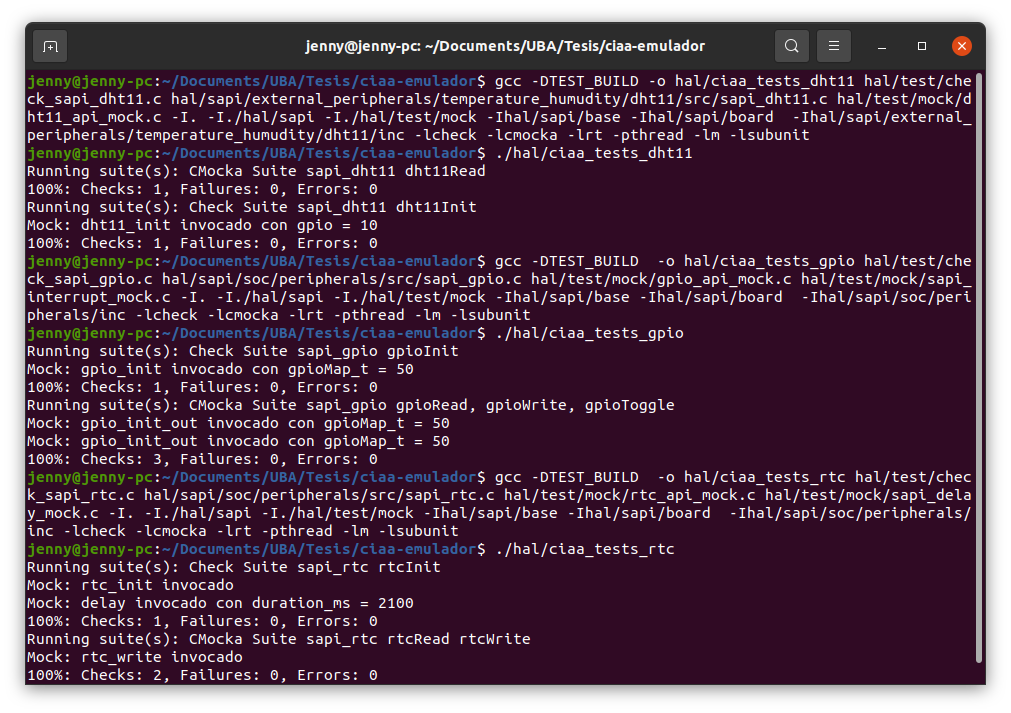
\includegraphics[scale=.27]{./Figures/PruebasUnidad1.png}
	\caption{Primera parte de la salida por consola de las pruebas unitarias con \textit{CMocka} o \textit{Check}.}
	\label{fig:PruebasUnidad1}
\end{figure}


\begin{figure}[ht]
	\centering
	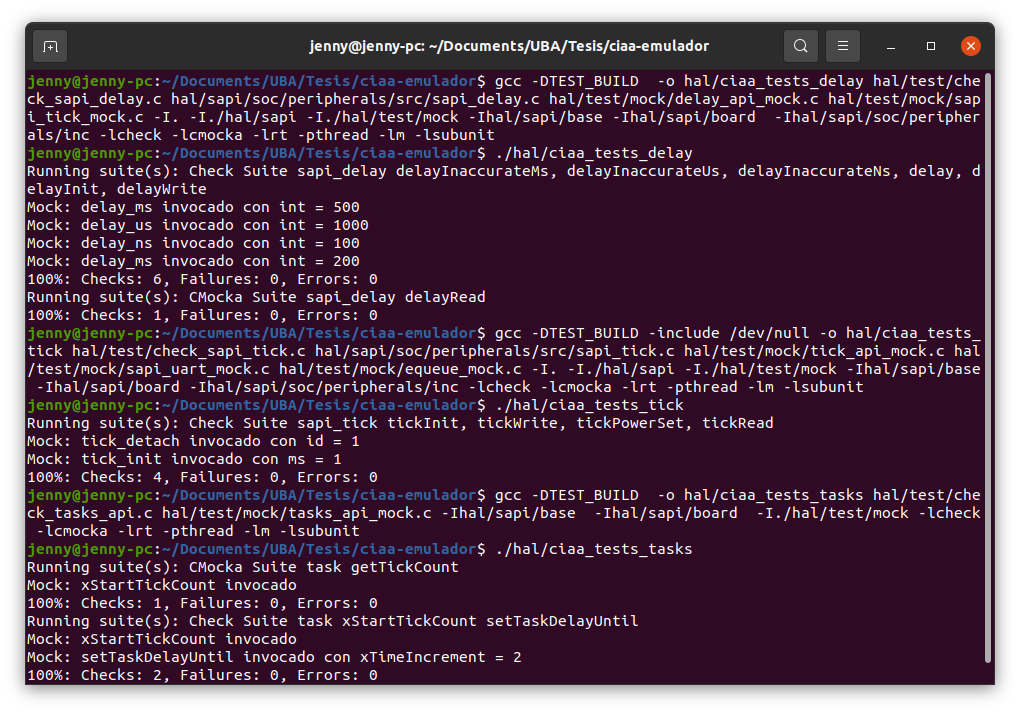
\includegraphics[scale=.27]{./Figures/PruebasUnidad2.png}
	\caption{Segunda parte de la salida por consola de las pruebas unitarias con \textit{CMocka} o \textit{Check}.}
	\label{fig:PruebasUnidad2}
\end{figure}
 

\section{Pruebas de Integración} 
\label{subsec:Pruebas de Integración}

Las pruebas de integración se centran en evaluar la interacción y comunicación entre diferentes componentes. Además, asegura que trabajen en conjunto sin problemas.

A medida que se fueron desarrollando diferentes módulos y funcionalidades del emulador, las pruebas de integración fueron necesarias para identificar posibles conflictos o incompatibilidades entre los distintos componentes de código del emulador web.

Se fueron identificando las interacciones entre componentes que fueron relevantes a partir de las pruebas de unidad existentes, como \texttt{sapi\_delay} y \texttt{sapi\_tick}. Luego, se identificaron las dependencias de \textit{Emscripten} y las funciones que se invocan entre las diferentes pruebas de unidad.

Luego, se crearon archivos de prueba de integración con escenarios especificos que combinen las interacciones entre los componentes y se utilizaron \textit{mocks} para simular comportamientos de funciones de \textit{Emscripten}.

Al igual que en las pruebas de unidad se utilizo el compilador GCC para compilar. A continuacion la figura \ref{fig:PruebasIntegracion} muestra los resultados por consola de las pruebas de integracion.

\begin{figure}[ht]
	\centering
	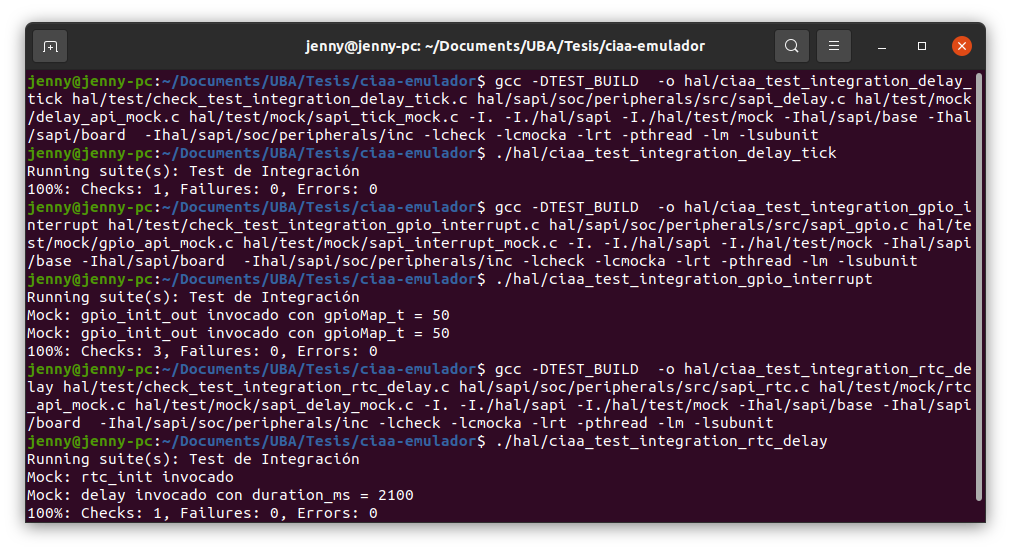
\includegraphics[scale=.35]{./Figures/PruebasIntegracion.png}
	\caption{Depuración de las pruebas de integracion.}
	\label{fig:PruebasIntegracion}
\end{figure}

\section{Pruebas de Interfaz}
\label{sec:Pruebas de Interfaz}

Para lograr que la interfaz de la plataforma de emulación cumpla con los requisitos funcionales y logre que los usuarios lo adopten con éxito fue necesario implementar las pruebas de la interfaz de usuario.

Por tanto, se implementaron pruebas automatizadas que verifiquen que el funcionamiento sea el correcto, tanto desde la interacción con el usuario así como también con las peticiones hacia el backend.

La implementación de estas pruebas automatizadas permitió que se  ejecuten de forma rápida y confiable de manera recurrente. 

Para automatizar las pruebas de la interfaz de usuario con \textit{\textbf{NodeJS}}, se utilizó en el desarrollo las bibliotecas \textit{\textbf{Mocha}} y \textit{\textbf{Chai}}, que permitieron crear pruebas de interfaz muy completas para el desarrollo en \textit{JavaScript}.

Además, permitió asegurar que cada componente de la interfaz funcione correctamente por separado. Incluso, verificó si el código en el navegador web devolvió los nombres de los módulos correctos, los tipos de parámetros previstos y el tipo de retorno esperado.

La figura \ref{fig:TestVS1} muestra la salida por consola durante la depuración de las pruebas de interfaz con \textit{\textbf{Mocha}}.


\begin{figure}[ht]
	\centering
	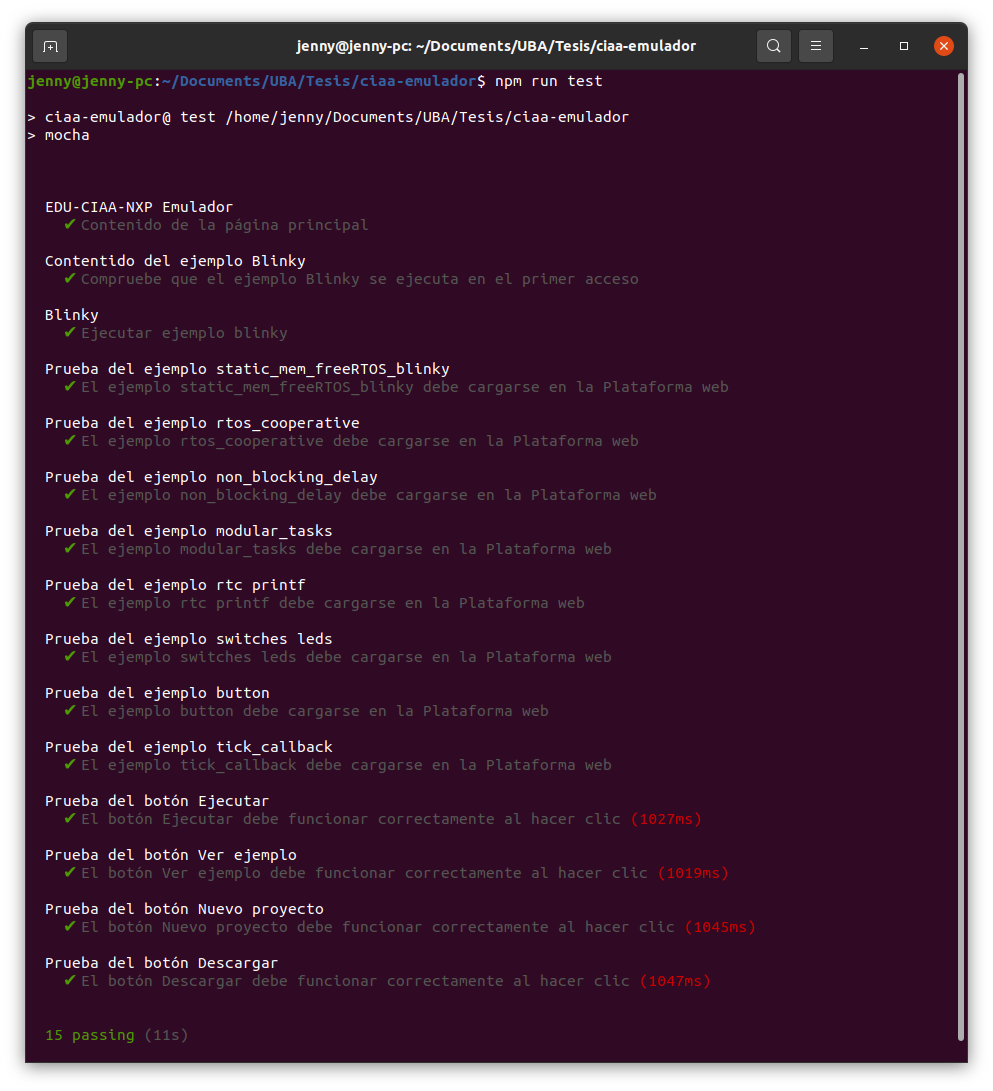
\includegraphics[scale=.29]{./Figures/TestInterfaz.png}
	\caption{Salida por consola durante la depuración de las pruebas de interfaz con \textit{\textbf{Mocha}}.}
	\label{fig:TestVS1}
\end{figure}

\section{Integracion Continua}
\label{sec:Integracion Continua}

En la realización de la integración continua, al principio no se tenía claro cuál herramienta utilizar. Como parte del proceso de análisis para el presente trabajo final, se investigaron las plataformas de GitLab CI y Travis CI y ambas herramientas, proporcionaron excelentes resultados y demostraron ser igualmente eficaces. Sin embargo, se encontraron algunas diferencias importantes en su configuración y en cómo se presentan las pruebas en cada plataforma.

En el caso de GitLab CI, toda la configuración se realizó directamente en la plataforma de GitLab, lo que facilitó la integración con el repositorio de la plataforma web y permitió una gestión más centralizada del proceso de CI/CD.

Por otro lado, con Travis CI, se realizaron configuraciones separadas de GitHub. Esto implicó un enfoque más descentralizado, lo que puede ser útil si se trabaja en varios proyectos alojados en diferentes repositorios.

Después de evaluar ambas opciones, se decidió continuar utilizando ambas tecnologías, ya que el esfuerzo para configurar ambas CI ya se realizó. Esta elección brindó mayor flexibilidad y resguardo en caso de problemas con alguna de estas herramientas.

En general, la experiencia con ambas herramientas fue positiva y permite mejorar la calidad y eficiencia del proceso de desarrollo mediante la automatización de las pruebas unitarias y de integracion, Además de los despliegues continuos.

En ambas plataformas, la información que se muestra en la consola proporciona la siguiente información útil:

\begin{itemize}
	\item Resultado de las pruebas: la consola muestra si las pruebas se ejecutaron con éxito o si hubo fallas en alguna de ellas. 
	
	\item Detalle de los fallos: en el caso de que alguna prueba falle, la consola proporcionará información detallada, como el nombre de la prueba, el nombre del archivo y la línea de código donde ocurrió el error.
	
	\item Información sobre el entorno de prueba: la consola muestra detalles sobre el entorno de prueba utilizado tanto en Travis CI  como en GitLab CI, que incluye la versión del lenguaje de programación, la secuencia de dependencias instaladas y otros detalles de las pruebas.
	
	\item Duración de las pruebas: la consola muestra el tiempo que tardaron todas las pruebas en ejecutarse,  de manera que, permite identificar las pruebas que deben ser modificadas para optimizar su rendimiento.
	
	\item Logs de ejecución: la consola mostrará registros detallados de la ejecución de las pruebas, que incluyen mensajes del progreso de las pruebas, información de depuración y los resultados de las pruebas.
	
\end{itemize}

La siguiente figura \ref{fig:travis} presenta la consola de Travis CI.  

\begin{figure}[ht]
	\centering
	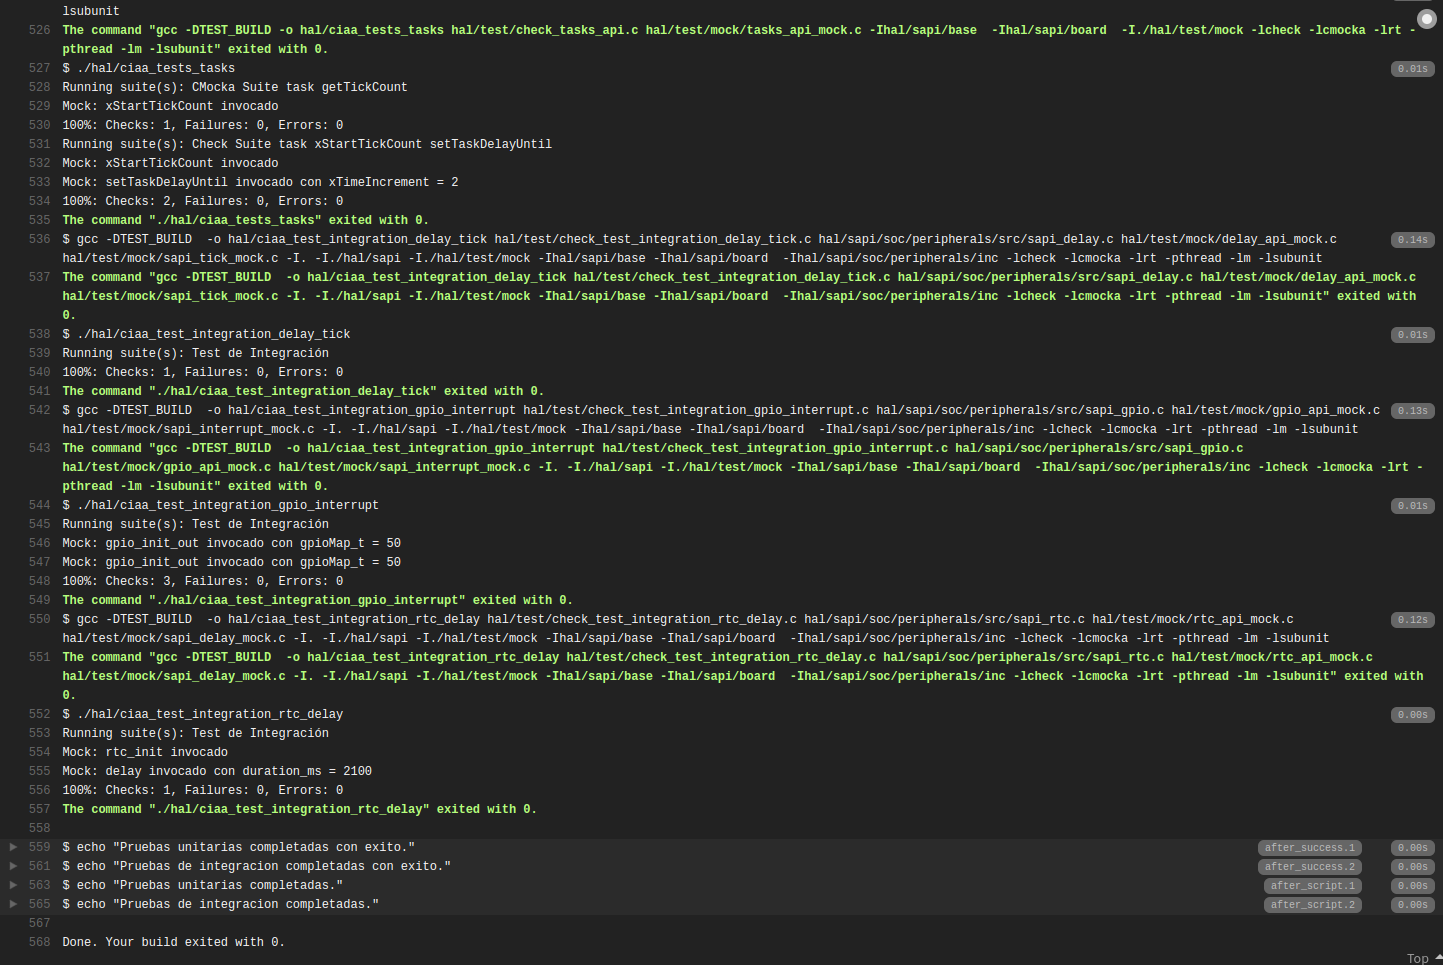
\includegraphics[scale=.35]{./Figures/travis.png}
	\caption{Información de las pruebas que se ejecutaron en Travis CI.}
	\label{fig:travis}
\end{figure}

\hfill \break
\hfill \break
\hfill \break
\hfill \break
\hfill \break
\hfill \break

La figura \ref{fig:gitLab} presenta la consola de GitLab CI.  

\begin{figure}[ht]
	\centering
	\includegraphics[scale=.40]{./Figures/gitLab.png}
	\caption{Información de las pruebas que se ejecutaron en GitLab CI.}
	\label{fig:gitLab}
\end{figure}

\subsection{Prueba de acceso}    

Para verificar y validar el acceso mediante solicitudes HTTP al servidor donde se encuentra publicado el emulador de la plataforma web, se utilizó la herramienta Postman.

Antes de comenzar con el ensayo, se creó un caso de prueba con el propósito de ser una guía estructurada y documentada para verificar si el acceso al servidor funciona como se espera.


\textit{\textbf{ID Caso de prueba: CP01}}

Descripción: la primera vez que el usuario ingresa a la plataforma de emulación se muestra en ejecución el ejemplo predeterminado \textit{Blinky}.

Pre-condición: 
\begin{itemize}
	\item La computadora del usuario tiene conexión a Internet y un navegador web instalado.
\end{itemize}

Flujo principal:
\begin{itemize}
	\item El usuario ingresa al entorno web de la plataforma de emulación para la placa EDU-CIAA-NXP.
\end{itemize}
Post condiciones:
\begin{itemize}
	\item ÉXITO: la plataforma muestra el ejemplo \textit{\textbf{Blinky}} en ejecución.
	\item FALLA: La plataforma no muestra ningún ejemplo predeterminado en ejecución.
\end{itemize}

Resumen del Test:
\begin{itemize}
	\item Después de acceder a la plataforma mediante los navegadores web Chrome, Firefox y Explorer se comprobó que se muestra en ejecución el ejemplo \textit{\textbf{Blinky}}.
	\item Se realizó la prueba de HTTP \textit{requests} por medio de la utilización de la herramienta \textit{\textbf{Postman}} que luego de acceder a la dirección del servidor donde se encuentra la plataforma, devolvió en formato \textit{\textbf{JSON}} la respuesta del servidor.
\end{itemize}


La figura \ref{fig:PlataformaEmuladorBlinky} muestra la plataforma de emulación ejecutando el ejemplo predeterminado \textit{\textbf{Blinky}}.

\begin{figure}[ht]
	\centering
	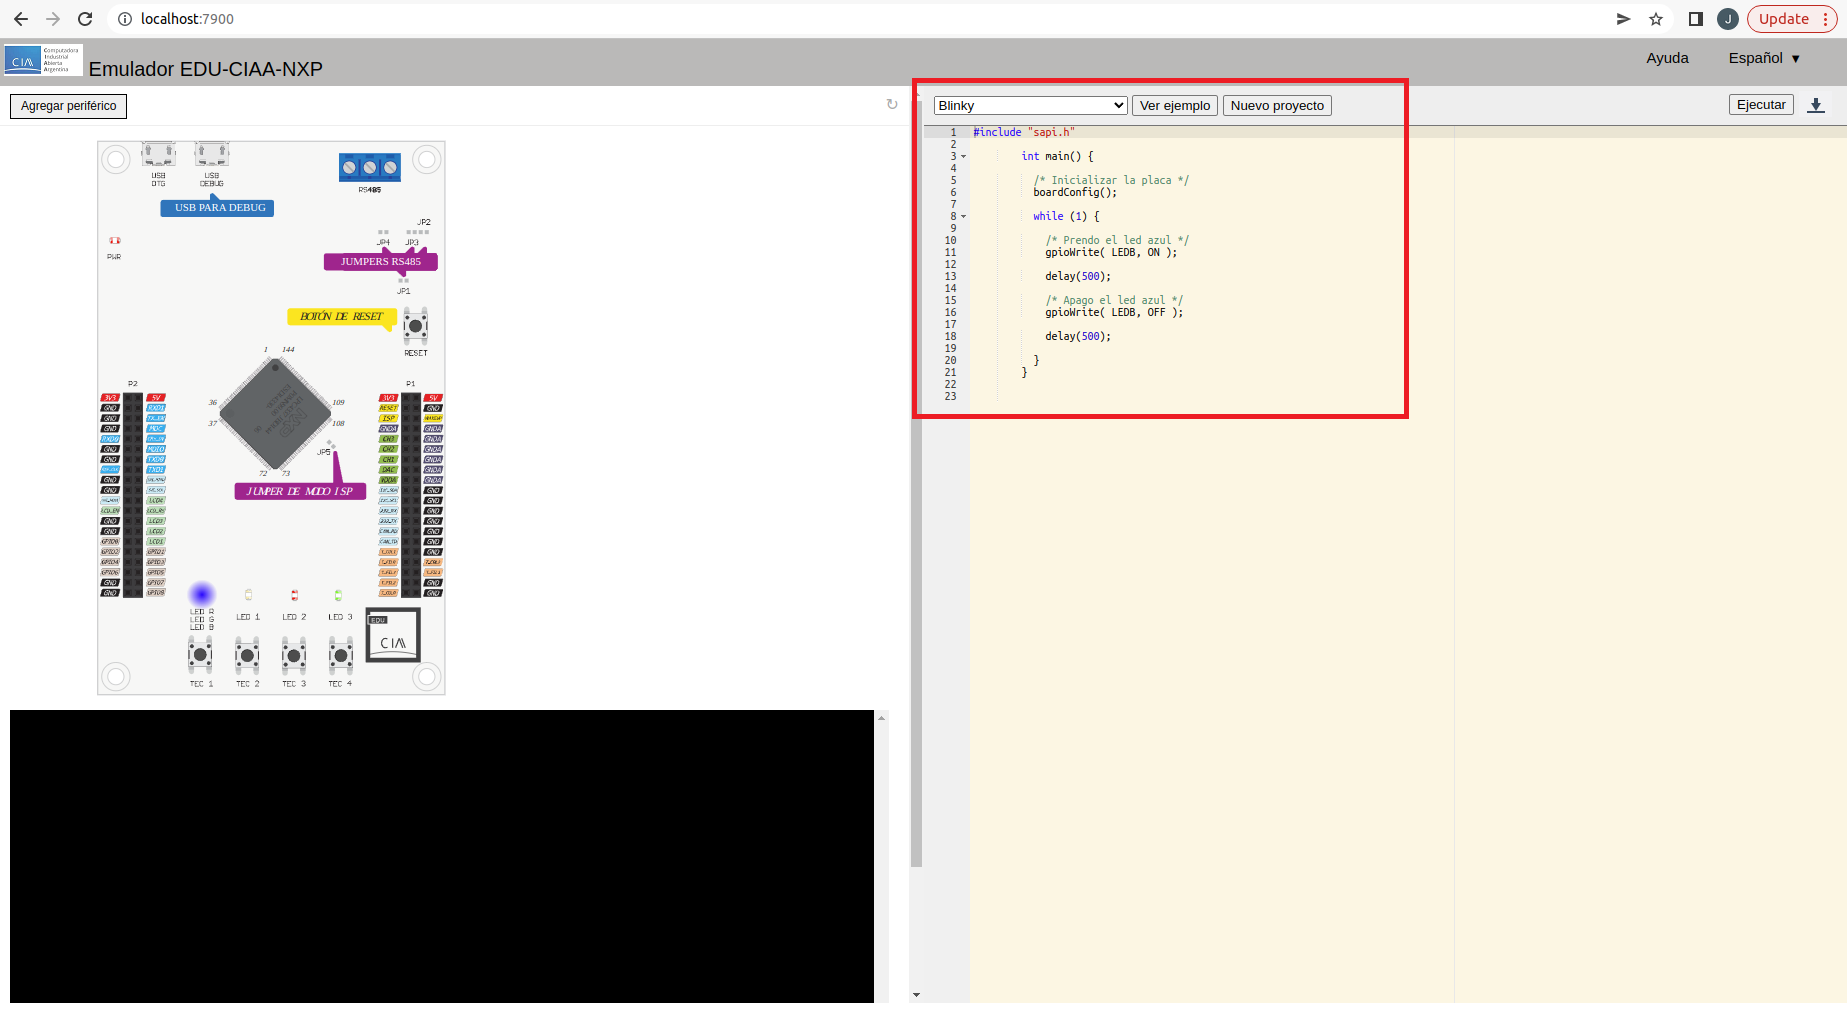
\includegraphics[scale=.28]{./Figures/PlataformaEmuladorBlinky.png}
	\caption{Prueba plataforma emulador ejecutando el ejemplo \textit{\textbf{Blinky}}.}
	\label{fig:PlataformaEmuladorBlinky}
\end{figure}

\textit{\textbf{Postman}} es una aplicación que permite realizar pruebas API. Con este cliente \textit{\textbf{HTTP}} se probó \textit{\textbf{HTTP requests}} que permitió el acceso al servidor de la plataforma de emulación y por medio de la cual se obtuvo la respuesta en diferentes formatos como  \textit{\textbf{JSON}}, \textit{\textbf{XML}}, \textit{\textbf{HTML}} y \textit{\textbf{Text}}.


En la figura \ref{fig:PostmanBlinky2} se muestra la petición y respuesta de acceso a la plataforma por medio de la herramienta \textit{\textbf{Postman}}.

\hfill \break
\hfill \break
\hfill \break
\hfill \break
\hfill \break
\hfill \break
\hfill \break

\begin{figure}[ht]
	\centering
	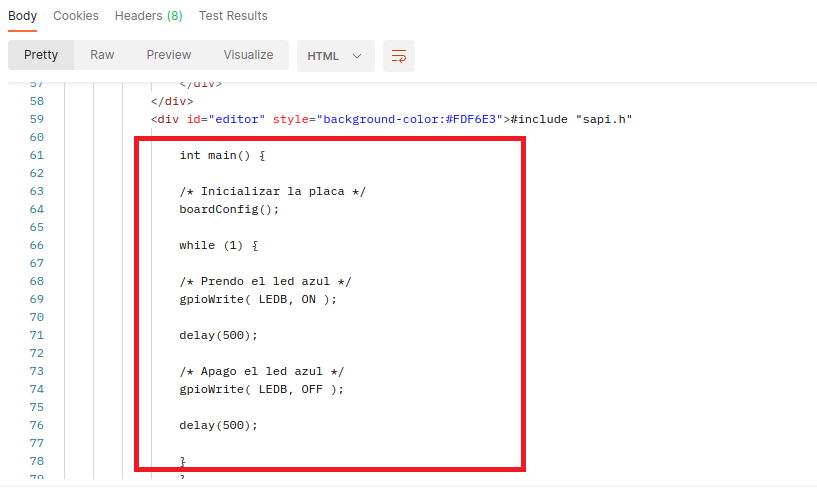
\includegraphics[scale=.37]{./Figures/PostmanBlinky2.png}
	\caption{Respuesta del servidor.}
	\label{fig:PostmanBlinky2}
\end{figure}



\section{Pruebas de funcionamiento}  
\label{sec:Pruebas de funcionamiento}
En las pruebas de funcionamiento en un entorno web de simulación de un microcontrolador, se evalúa y verifica el comportamiento y desempeño de la simulación del microcontrolador en el entorno web. Estas pruebas son esenciales para asegurar que la simulación se comporte adecuadamente y funcione correctamente en el contexto en el que se está utilizando.

Comparar la precisión de los cálculos realizados por el microcontrolador en la plataforma web con los resultados obtenidos en la placa física.

\subsection{Prueba \textit{\textbf{Dht11 temperature/humidity}} }

\subsubsection{Ensayo en la plataforma de emulación para la placa EDU-CIAA-NXP} 
Para el ensayo en la plataforma de emulación web se siguió con los pasos del siguiente caso de uso:

\textit{\textbf{ID Caso de prueba: CP02}}

Descripción: la plataforma de emulación permite al usuario ejecutar el ejemplo \textit{\textbf{Dht11 temperature/humidity}}.

Pre-condición: 
\begin{itemize}
	\item La computadora del usuario tiene conexión a Internet y un navegador web instalado.
\end{itemize}

Flujo principal:
\begin{enumerate}
	\item El usuario ingresa al entorno web de la plataforma de emulación para la placa EDU-CIAA-NXP.
	\item El usuario selecciona desde la lista desplegable el ejemplo \textit{\textbf{Dht11 temperature/humidity}} y hace click en el botón \textquotedbl Ver ejemplo \textquotedbl.
	\item La plataforma muestra en pantalla al usuario el código del ejemplo \textit{\textbf{Dht11 temperature/humidity}}.
	\item El usuario hace clic en la imagen del periférico DHT11 en la barra lateral (sidebar) del área de ensamblado, donde se muestran los periféricos disponibles en la plataforma web.
	\item La plataforma muestra al usuario una ventana con las conexiones correctas por defecto del sensor \textit{\textbf{Dht11 temperature/humidity}}.
	\item El usuario hace click en el botón \textquotedbl Agregar \textquotedbl.
	\item La plataforma muestra integrado el componente \textit{\textbf{Dht11 temperature/humidity}} con la opción por defecto \textquotedbl Obtener temperatura local del servidor climático \textquotedbl, junto a la placa EDU-CIAA-NXP.
	\item El usuario hace click en el botón \textquotedbl Ejecutar \textquotedbl.
	\item La plataforma muestra en la consola integrada la salida de la temperatura y humedad con los valores enviados desde la central meteorológica en línea.
\end{enumerate}

Flujo alternativo:
\begin{enumerate}
    \setcounter{enumi}{7}
	\item El usuario hace clic en la opción \textquotedbl Establecer temperatura y humedad manualmente \textquotedbl y comienza a manipular los termómetros gráficos haciendo clic sobre los que corresponden a la temperatura y a la humedad.
	\item La interfaz deselecciona la opción \textquotedbl Obtener temperatura local del servidor climático \textquotedbl y muestra seleccionada la opción \textquotedbl Establecer temperatura y humedad manualmente \textquotedbl.
	\item El usuario hace click en el botón \textquotedbl Ejecutar \textquotedbl.
	\item La plataforma muestra en la consola integrada la salida de la temperatura y humedad con los valores elegidos por el usuario desde los termómetros gráficos.
\end{enumerate}



Post condiciones:
\begin{itemize}
	\item ÉXITO: la plataforma muestra en ejecución el ejemplo \textit{\textbf{Dht11 temperature/humidity}}.
	\item FALLA: La plataforma no muestra al usuario ningún cambio en la consola.
\end{itemize}



Luego de completar el caso de uso CP02 con: flujo principal y flujo alternativo, se obtuvo el siguiente resultado: 

\begin{itemize}
	\item ÉXITO: la plataforma muestra en ejecución el ejemplo \textit{\textbf{Dht11 temperature/humidity}}.
\end{itemize}

La figura \ref{fig:RespuestaEmulador} muestra la consola con los datos de temperatura y humedad del ejemplo \textit{\textbf{Dht11 temperature/humidity}} con la opción \textquotedbl Obtener temperatura local del servidor climático \textquotedbl.

\hfill \break
\hfill \break
\hfill \break

\begin{figure}[ht]
	\centering
	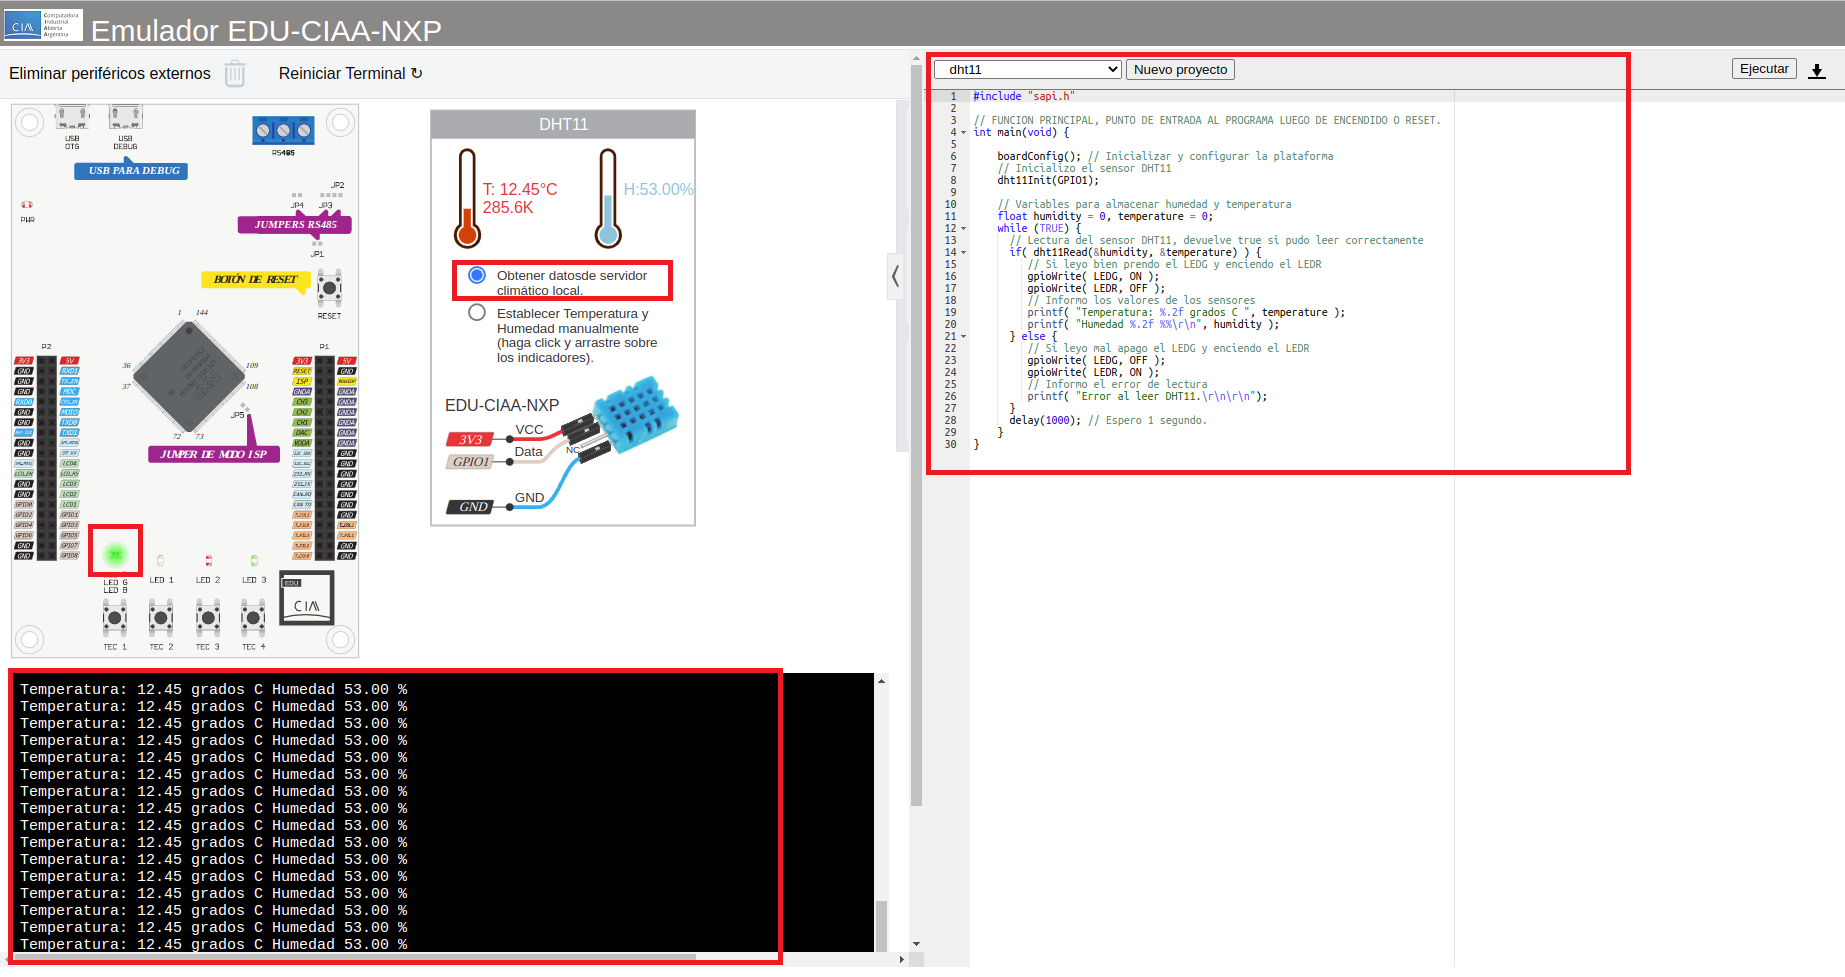
\includegraphics[scale=.28]{./Figures/dht11Opcion1.png}
	\caption{La plataforma muestra el resultado del CP02.}
	\label{fig:RespuestaEmulador}
\end{figure}


La figura \ref{fig:RespuestaEmulador} muestra la consola con los datos de temperatura y humedad del ejemplo \textit{\textbf{Dht11 temperature/humidity}} con la opción \textquotedbl Establecer temperatura y humedad manualmente \textquotedbl.


\begin{figure}[ht]
	\centering
	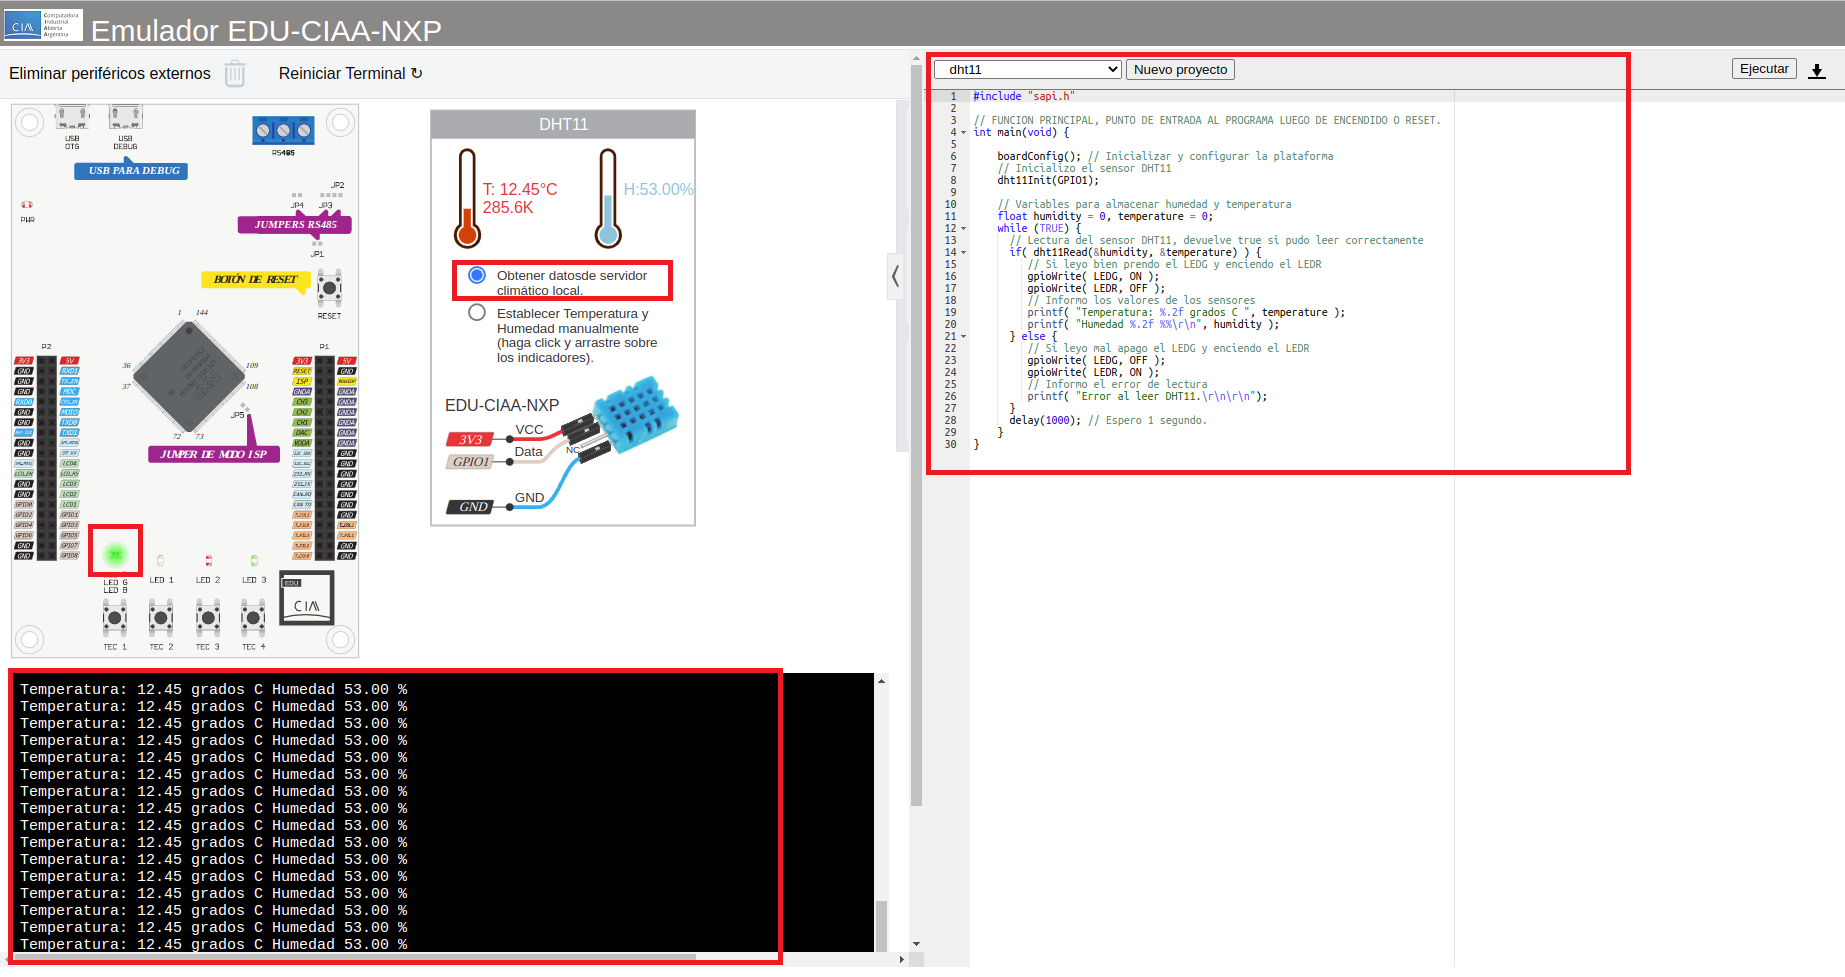
\includegraphics[scale=.28]{./Figures/dht11Opcion1.png}
	\caption{La plataforma muestra el resultado del CP02.}
	\label{fig:RespuestaEmulador}
\end{figure}




Para verificar que la plataforma obtuvo los datos de temperatura/humedad del API de meteorología  \textit{\textbf{openweathermap}} se hicieron pruebas de request con la herramienta \textit{Postman}.

En la figura \ref{fig:RespuestaPostMan1} se observa que la petición de datos de temperatura/humedad recibe como parámetro la ciudad que se quiere consultar.

\hfill \break


\begin{figure}[ht]
	\centering
	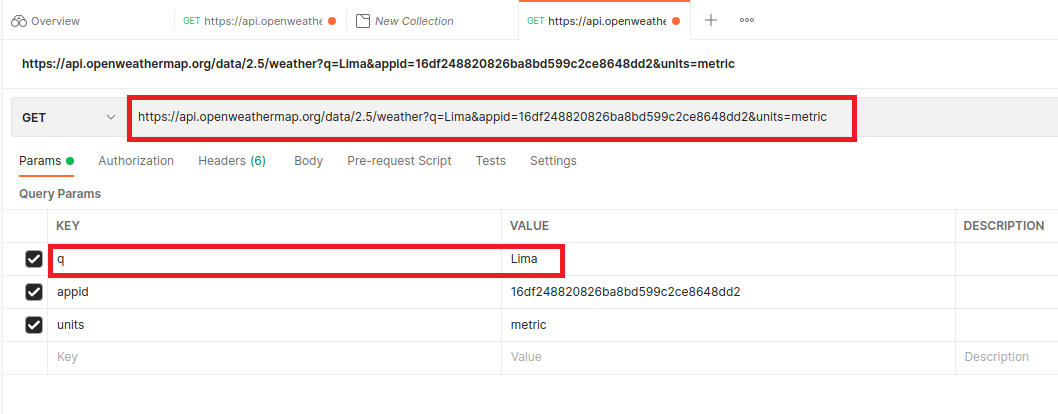
\includegraphics[scale=.30]{./Figures/RespuestaPostMan1.png}
	\caption{Petición de datos de temperatura/humedad.}
	\label{fig:RespuestaPostMan1}
\end{figure}

En este paso se verifica que la respuesta de la petición de datos de temperatura/humedad al API \textit{\textbf{openweathermap}} coincide con lo que se observó en la terminal de la plataforma de emulación.


\subsubsection{Ensayo en la plataforma EDU-CIAA-NXP} 

Este ensayo tuvo como objetivo identificar
las diferencias entre los resultados reales producidos por la placa real y los resultados esperados en la plataforma de emulación.

El primer paso fue conectar el componente Dht11 a la placa EDU-CIAA-NXP. En consecuencia, se procedió a compilar el ejemplo \textit{\textbf{Dht11 temperature/humidity}} de la plataforma de emulación dentro de la herramienta 
\textit{Eclipse} y luego, se grabó en la placa EDU-CIAA-NXP.

A continuación se muestra en la figura \ref{fig:TestHardware} la ejecución del ensayo en la plataforma EDU-CIAA-NXP.

\begin{figure}[ht]
	\centering
	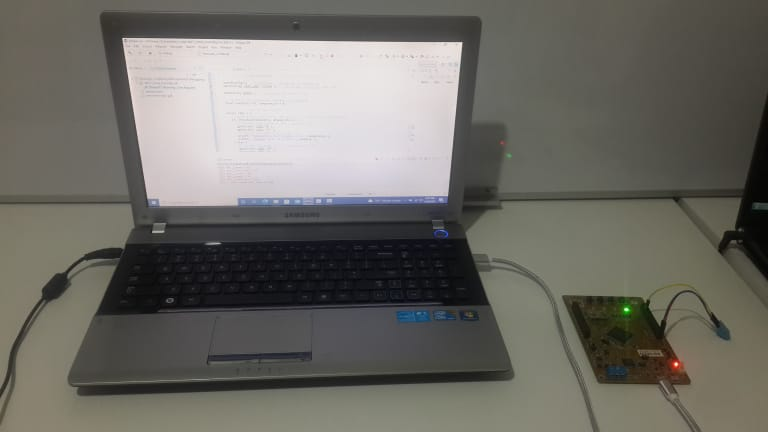
\includegraphics[scale=.49]{./Figures/TestHardware.jpeg}
	\caption{Ensayo del ejemplo \textit{\textbf{Dht11 temperature/humidity}}.}
	\label{fig:TestHardware}
\end{figure}



La figura \ref{fig:TestEclipse} muestra el código del ejemplo \textit{\textbf{Dht11 temperature/humidity}} en la herramienta \textit{eclipse} de la PC de prueba.

\begin{figure}[ht]
	\centering
	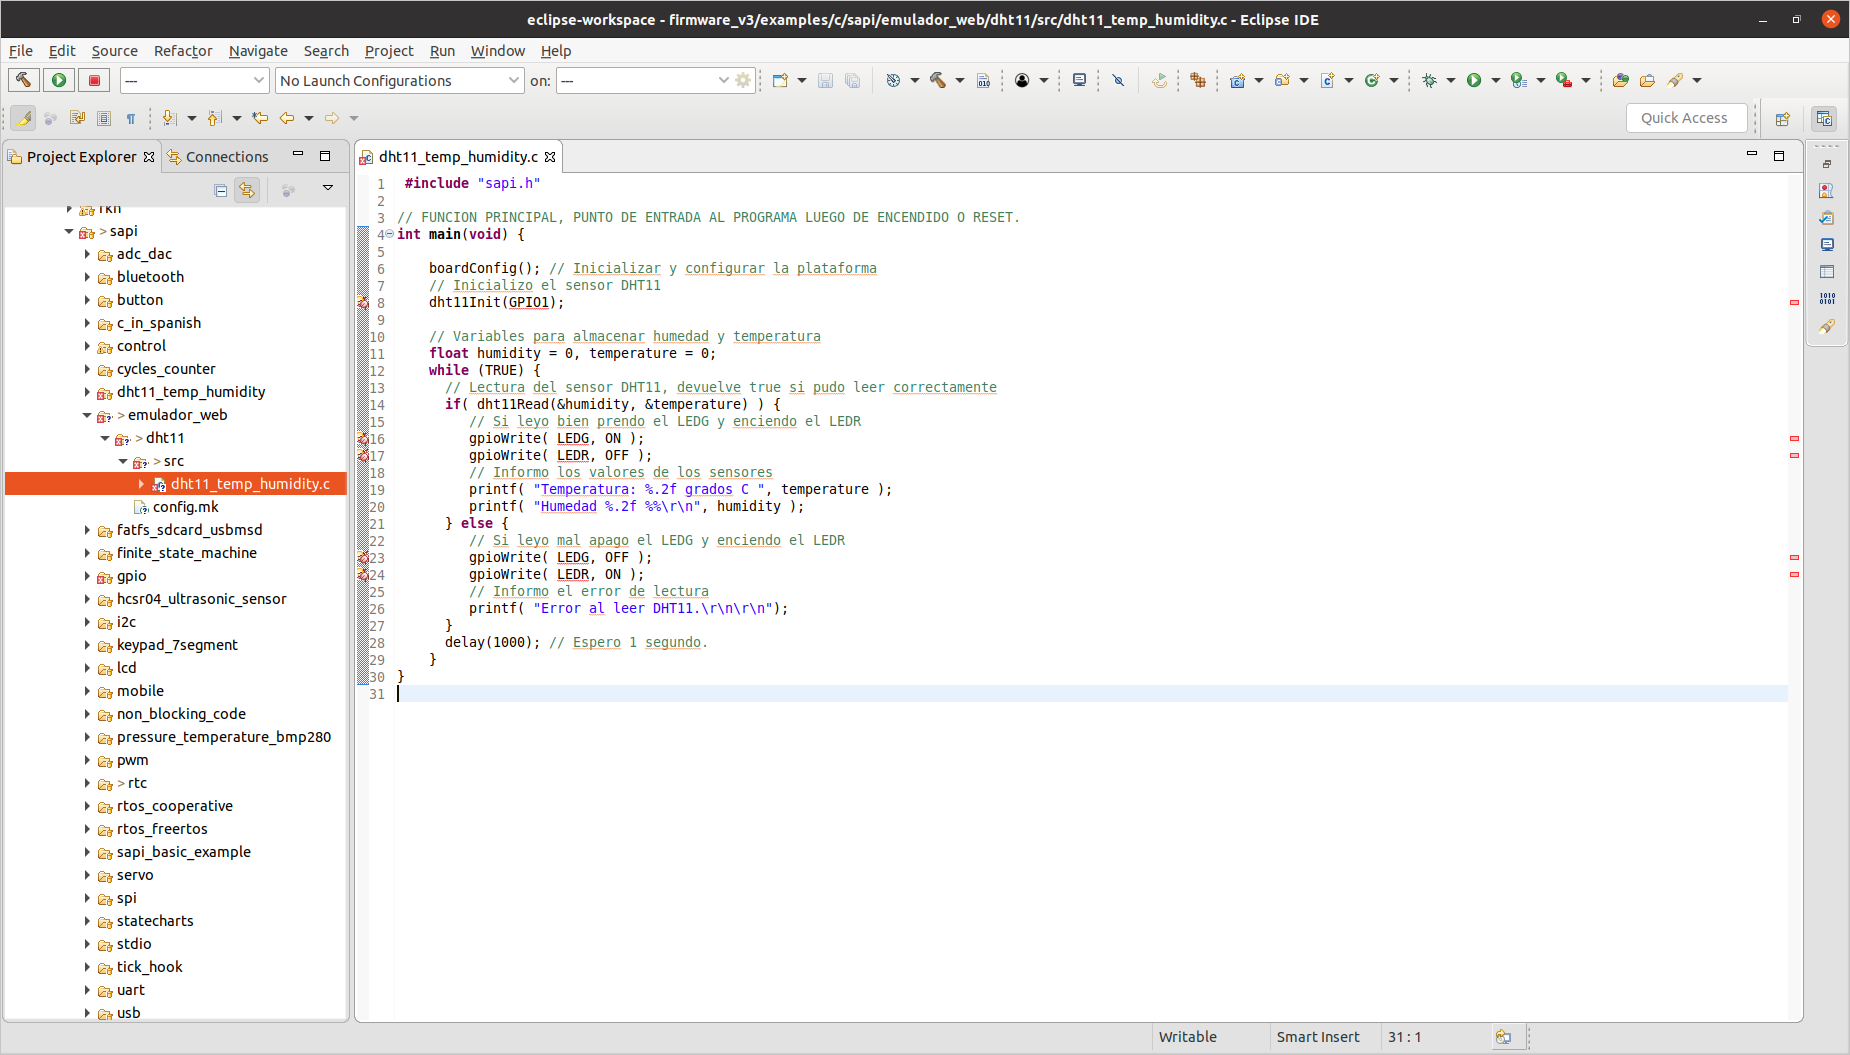
\includegraphics[scale=.22]{./Figures/TestEclipse.png}
	\caption{Código del ejemplo en eclipse.}
	\label{fig:TestEclipse}
\end{figure}


El programa \textit{\textbf{Dht11 temperature/humidity}} de la plataforma de emulación es un ejemplo simple que solo enciende el LEDG en la placa y además, lee los datos generados del sensor Dht11 que consisten en temperatura/humedad. Luego, los datos leídos se imprimen por pantalla. 

En este ensayo manual se registraron los cambios en la placa y también, los mensajes de la terminal serie. De modo que, posteriormente, permitió compararlos con la plataforma de emulación.

En la figura \ref{fig:TestPlaca} se observan los cambios en la placa que fueron registrados durante las pruebas.


\begin{figure}[ht]
	\centering
	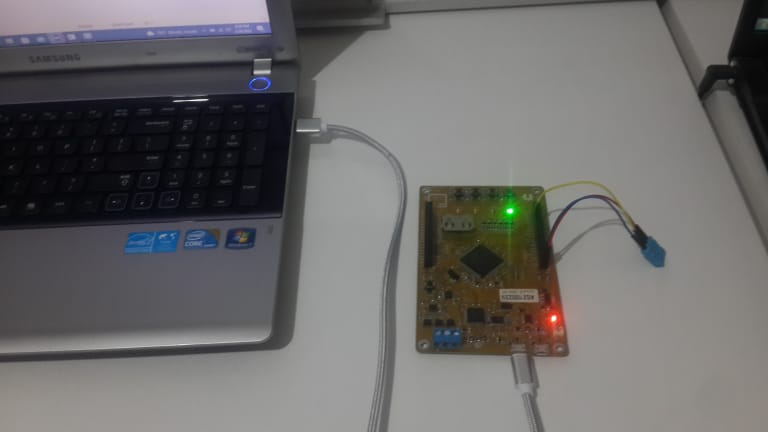
\includegraphics[scale=.50]{./Figures/TestPlaca.jpeg}
	\caption{Cambios en la placa EDU-CIAA-NXP durante el ensayo.}
	\label{fig:TestPlaca}
\end{figure}


Ahora bien, para leer los datos por pantalla se utilizó la herramienta \textit{Tera Term VT} que permitió levantar los datos de temperatura/humedad.

En la figura \ref{fig:TestTerminal} se muestra los datos de temperatura/humedad usando \textit{Tera Term VT}. 


\begin{figure}[ht]
	\centering
	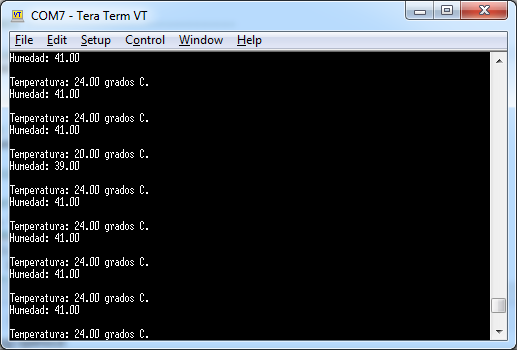
\includegraphics[scale=.80]{./Figures/TestTerminal.png}
	\caption{Salida de la terminal COM7 -Tera Term VT.}
	\label{fig:TestTerminal}
\end{figure}



Resumen del Test:
\begin{itemize}
	\item Después de acceder a la plataforma mediante el navegador y siguiendo los pasos del flujo principal y el flujo alternativo de la prueba, se comprobó que se muestra en ejecución el ejemplo \textit{\textbf{Dht11 temperature/humidity}}.
	\item Se realizó la prueba de HTTP \textit{requests} usando la herramienta \textit{\textbf{Postman}} para comprobar la respuesta del \textit{\textbf{API openweathermap}} que consume la plataforma de emulación de manera que, los datos de temperatura y humedad sean los mismos.
	\item Se ensayo en la placa real EDU-CIAA-NXP  el mismo ejemplo \textit{\textbf{Dht11 temperature/humidity}} y se registraron los resultados de la terminal serial.

\end{itemize}


\subsection{ Prueba \textit{\textbf{tick hook}}}
El objetivo de este ensayo es exponer las diferencias en los resultados encontrados entre el emulador web y la placa fisica.

\subsubsection{Ensayo en la plataforma de emulación para la placa EDU-CIAA-NXP} 
Para ensayar la plataforma web, se ejecuto el siguiente caso de uso:

\textit{\textbf{ID Caso de prueba: CP03}}

Descripción: la plataforma de emulación permite al usuario ejecutar un nuevo ejemplo de \textit{\textbf{tick hook}}.

Pre-condición: 
\begin{itemize}
	\item La computadora del usuario tiene conexión a Internet y un navegador web instalado.
\end{itemize}

Flujo principal:
\begin{enumerate}
	\item El usuario ingresa al entorno web de la plataforma de emulación para la placa EDU-CIAA-NXP.
	\item El usuario hace click en el botón \textquotedbl Nuevo Proyecto \textquotedbl.
	\item La plataforma muestra en pantalla al usuario el area de codificacion listo para que pueda ingresar su propio codigo.
	\item El usuario ingresa el siguiente codigo de prueba:
	
\begin{lstlisting}[caption={nuevo proyecto}]
#include "sapi.h"

void myTickHook( void *ptr )
{
   gpioWrite( LED3, ON );
   printf( "Blinky LED3.\r\n" );
   while(TRUE) {
      printf( " while(TRUE)  Blinky LED1.\r\n" );
      gpioToggle( LED1 );
      delay(1);
   }
}

int main()
{
    boardConfig();
    tickInit(50);
    while ( TRUE )
    {
		tickCallbackSet( myTickHook, NULL );
		delay(5000);
    }
    return 0;
}
\end{lstlisting}

	\item El usuario hace click en el botón \textquotedbl Ejecutar \textquotedbl.
	\item La plataforma muestra en la consola integrada la salida del programa en ejecución.
	
\end{enumerate}
	

La figura \ref{fig:Testtickhook} muestra que la plataforma web muestra en la consola integrada la salida de \textquotedbl Blinky LED3 \textquotedbl muchas veces. 

\hfill \break
\hfill \break
\hfill \break
\hfill \break
\hfill \break
\hfill \break
\hfill \break
\hfill \break
\hfill \break
\hfill \break
\hfill \break

\begin{figure}[ht]
	\centering
	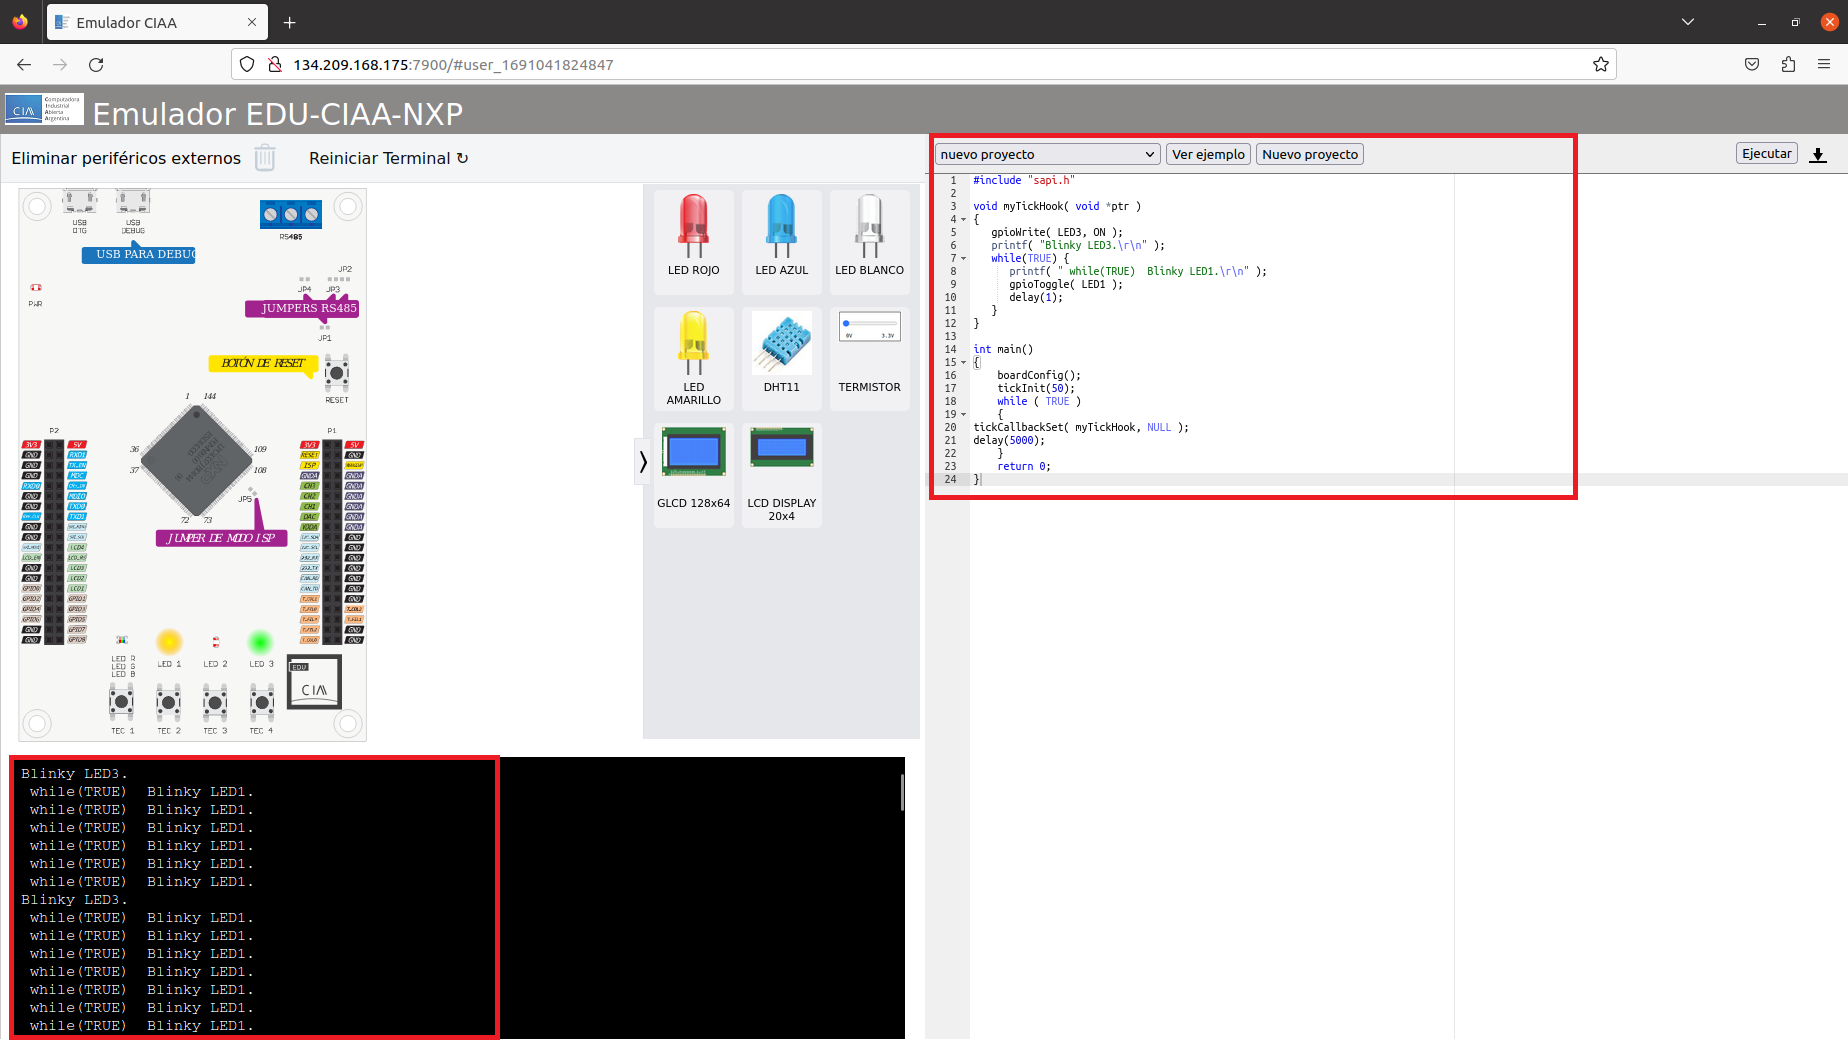
\includegraphics[scale=.25]{./Figures/Testtickhook.png}
	\caption{Salida por consola del ensayo tick hook.}
	\label{fig:Testtickhook}
\end{figure}

\subsubsection{Ensayo en la plataforma EDU-CIAA-NXP} 

Se ejecuta el mismo ejemplo en la placa fisica y se obtiene por consola la siguiente salida que se muestra en la siguiente figura \ref{fig:TesttickhookPlaca}:



\begin{figure}[ht]
	\centering
	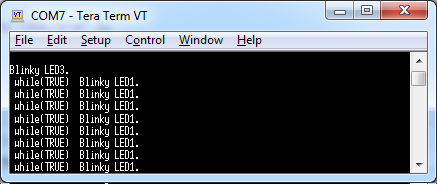
\includegraphics[scale=.80]{./Figures/TesttickhookPlaca.png}
	\caption{Salida de la terminal COM7 -Tera Term VT.}
	\label{fig:TesttickhookPlaca}
\end{figure}

Se observa que la salida por consola de \textquotedbl Blinky LED3 \textquotedbl se muestra solo una vez, lo cual difiere de la salida por consola de la plataforma web que muestra \textquotedbl Blinky LED3 \textquotedbl muchas veces.

\subsection{ Prueba \textit{\textbf{rtc printf}}}

Para el ensayo en la plataforma de emulación web se siguió con los pasos del siguiente caso de uso:

\textit{\textbf{ID Caso de prueba: CP04}}

Descripción: la plataforma de emulación permite al usuario ejecutar el ejemplo \textit{\textbf{rtc printf}}.

Pre-condición: 
\begin{itemize}
	\item La computadora del usuario tiene conexión a Internet y un navegador web instalado.
\end{itemize}

Flujo principal:
\begin{enumerate}
	\item El usuario ingresa al entorno web de la plataforma de emulación para la placa EDU-CIAA-NXP.
	\item El usuario selecciona desde la lista desplegable el ejemplo \textit{\textbf{rtc printf}} y hace click en el botón \textquotedbl Ver ejemplo \textquotedbl.
	\item La plataforma muestra en pantalla al usuario el código del ejemplo \textit{\textbf{rtc printf}}.
	\item El usuario hace click en el botón \textquotedbl Ejecutar \textquotedbl.
	\item La plataforma muestra en la consola integrada la salida del rtc.
\end{enumerate}


Post condiciones:
\begin{itemize}
	\item ÉXITO: la plataforma muestra en ejecución el ejemplo \textit{\textbf{rtc printf}}.
	\item FALLA: La plataforma no muestra al usuario ningún cambio en la consola.
\end{itemize}



Luego de completar el caso de uso CP04, se obtuvo el siguiente resultado: 

\begin{itemize}
	\item ÉXITO: la plataforma muestra en ejecución el ejemplo \textit{\textbf{rtc printf}}.
\end{itemize}


La figura \ref{fig:rtcprintf} muestra que la plataforma web muestra en la consola integrada la salida del ensayo . 

\begin{figure}[ht]
	\centering
	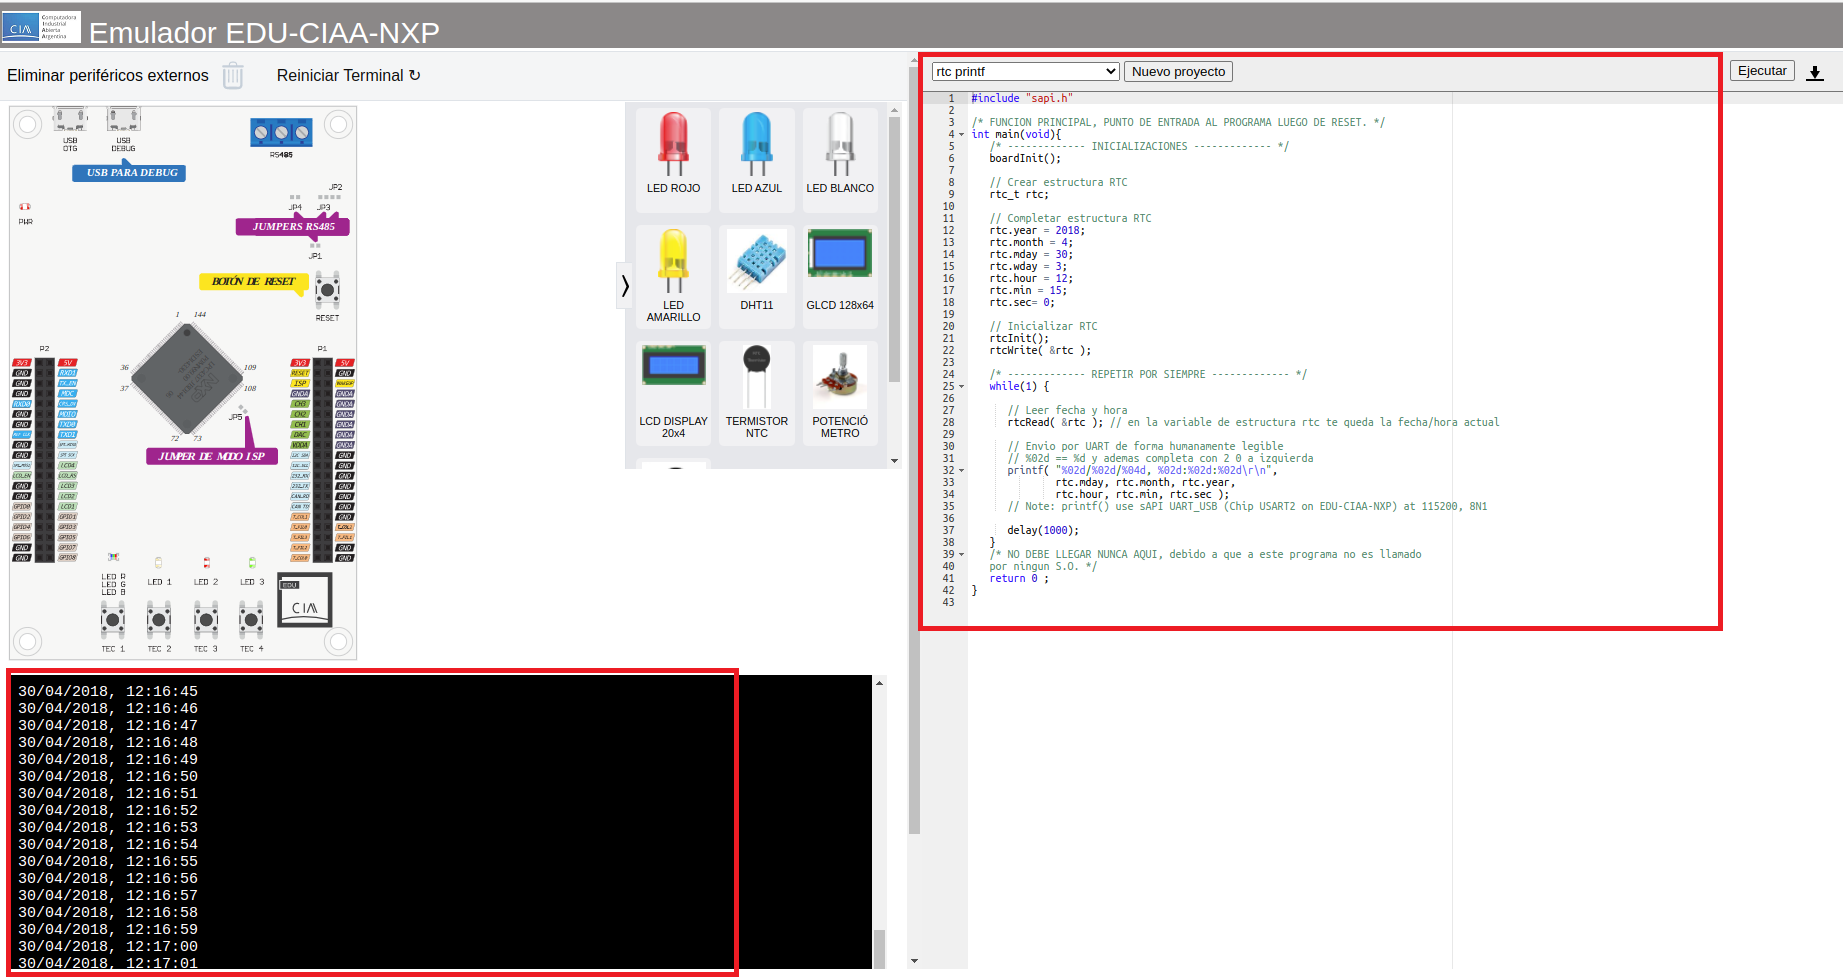
\includegraphics[scale=.28]{./Figures/rtcprintf.png}
	\caption{Salida por consola del ensayo rtc printf.}
	\label{fig:rtcprintf}
\end{figure}

\subsubsection{Ensayo en la plataforma EDU-CIAA-NXP} 

Se ejecuta el mismo ejemplo en la placa fisica y se obtiene por consola la siguiente salida que se muestra en la siguiente figura:

\begin{figure}[ht]
	\centering
	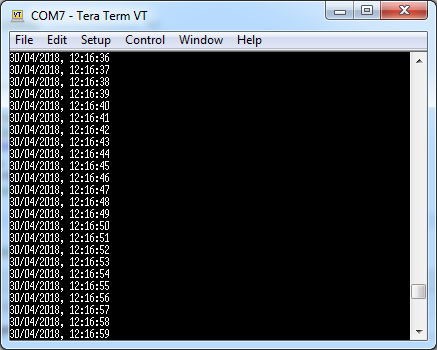
\includegraphics[scale=.90]{./Figures/rtcprintfPlaca.png}
	\caption{Salida de la terminal COM7 -Tera Term VT.}
	\label{fig:rtcprintfPlaca}
\end{figure}
